%% LyX 2.3.5-1 created this file.  For more info, see http://www.lyx.org/.
%% Do not edit unless you really know what you are doing.
\documentclass[a4paper,english]{article}
\usepackage[T1]{fontenc}
\usepackage[latin9]{inputenc}
\usepackage{babel}
\usepackage{units}
\usepackage{amsmath}
\usepackage{amssymb}
\usepackage{graphicx}
\usepackage[unicode=true]
 {hyperref}

\makeatletter

%%%%%%%%%%%%%%%%%%%%%%%%%%%%%% LyX specific LaTeX commands.
\pdfpageheight\paperheight
\pdfpagewidth\paperwidth


%%%%%%%%%%%%%%%%%%%%%%%%%%%%%% User specified LaTeX commands.
%\IEEEoverridecommandlockouts

\makeatother

\begin{document}
\title{Robust k-means method based on minimizing differentiable estimates of mean, insensitive to outliers}

\author{...}

%\author{
%\IEEEauthorblockN{%
%1\textsuperscript{st} Z.M.~Shibzukhov%
%}
%\IEEEauthorblockA{
%\textit{Institute Mathematics and %Informatics}\\%
%\textit{Moscow Pedagogical State %Univercity}\\%
%Moscow, Russia\\%
%szport@gmail.com%
%}\and
%\IEEEauthorblockN{%
%2\textsuperscript{nd} M.A.~Kazakov%
%}
%\IEEEauthorblockA{%
%\textit{Institute Applied Mathematics and %Automation}\\%
%\textit{Kabardino-Balkarian Scientific %Center RAS}\\%
%Nalchik, Russia\\%
%micro7777@mail.ru%
%} \and
%\IEEEauthorblockN{%
%3\textsuperscript{rd} %D.P.~Dimitrichenko%
%}
%\IEEEauthorblockA{
%\textit{Institute Applied Mathematics and %Automation}\\%
%\textit{Kabardino-Balkarian Scientific %Center RAS}\\%
%Nalchik, Russia\\%
%dimdp@rambler.ru%
%}%
%}

\maketitle
\begin{abstract}
A new approach to constructing a variant of the k-means clustering
algorithm is proposed, in which the Mahalanobis distance is used instead
of the Euclidean distance. It is based on minimizing differentiable
estimates of the mean, insensitive to outliers. The examples show
the possibility of stability of the proposed algorithm with respect
to outliers in the data.
\end{abstract}
robust clustering, robust mean estimate, iteratively reweighted algorithm.

\section{Introduction}

The problem of searching for cluster centers has been in the field
of attention of researchers for many years~\cite{cp1,cp2,cp3}.

The classical method for searching for centers and covariance matrices
of clusters can be based on solving the following minimization problem:
\begin{equation}
\mathbf{c}_{1}^{*},\dots,\mathbf{c}_{K}^{*}=\arg\min_{\mathbf{c}_{1},\dots,\mathbf{c}_{K}}\frac{1}{N}\sum_{k=1}^{N}\min_{j=1,\dots,K}d(\mathbf{x}_{k};\mathbf{c}_{j},\mathbf{S}_{j}),\label{eq:km_s}
\end{equation}
where $\mathbf{c}_{1},\dots,\mathbf{c}_{K}$ are cluster centers,
$\mathbf{S}_{1},\dots,\mathbf{S}_{K}$ are covariance matrices, 
\[
d(\mathbf{x};\mathbf{c},\mathbf{S})=\ln|\mathbf{S}|+(\mathbf{x}-\mathbf{c})^{\prime}\mathbf{S}^{-1}(\mathbf{x}-\mathbf{c})
\]
is the square of the Mahalanobis distance with the covariance matrix
$\mathbf{S}$ between the points $\mathbf{x}$ and $\mathbf{c}$.

This statement of the problem is based on the assumption that the
points of the $j$-th cluster obey a multidimensional normal distribution
with a density
\[
p(\mathbf{x};\mathbf{c},\mathbf{S})\propto\frac{1}{\sqrt{|\mathbf{S}|}}e^{-\frac{1}{2}(\mathbf{x}-\mathbf{c})^{\prime}\mathbf{S}^{-1}(\mathbf{x}-\mathbf{c})},
\]
an arbitrary point $\mathbf{x}$ refers to the cluster with the number
\[
j(\mathbf{x})=\arg\max_{j=1,\dots,K}p(\mathbf{x};\mathbf{c}_{j},\mathbf{S}_{j}).
\]

The problem \eqref{eq:km_s} is reduced to solving systems of equations:

\begin{equation}
\left\{ \begin{array}{l}
\mathbf{c}_{j}={\displaystyle \frac{1}{|\mathbf{I}_{j}|}\sum\limits _{k\in\mathbf{I}_{j}}\mathbf{x}_{k}}\\
\mathbf{S}_{j}={\displaystyle \frac{1}{|\mathbf{I}_{j}|}\sum\limits _{k\in\mathbf{I}_{j}}(\mathbf{x}_{k}-\mathbf{c}_{j})^{\prime}(\mathbf{x}_{k}-\mathbf{c}_{j})},
\end{array}\right.\label{eq:c_S_classic}
\end{equation}
where $\mathbf{I}_{j}\subset\{1,\dots,N\}$ are indices of points
falling into the $j$-th cluster.

The following iterative procedure underlies the extended \textsf{k-means}
algorithm:
\begin{equation}
\left\{ \begin{array}{l}
\mathbf{c}_{j,t+1}={\displaystyle \frac{1}{|\mathbf{I}_{j,t}|}\sum\limits _{k\in\mathbf{I}_{j,t}}\mathbf{x}_{k}}\\
\mathbf{S}_{j,t+1}={\displaystyle \frac{1}{|\mathbf{I}_{j,t}|}\sum\limits _{k\in\mathbf{I}_{j,t}}(\mathbf{x}_{k}-\mathbf{c}_{j,t})^{\prime}(\mathbf{x}_{k}-\mathbf{c}_{j,t})},
\end{array}\right.\label{eq:kmeans_alg}
\end{equation}
where $\mathbf{I}_{j,t}$ are indices of points falling into the $j$-th
cluster at the $t$-th step. Initial values of cluster centers $\mathbf{c}_{1,0},\dots,\mathbf{c}_{K,0}$
and covariance matrices $\mathbf{S}_{1,0},\dots,\mathbf{S}_{K,0}$
are set before the iteration procedure~\eqref{eq:kmeans_alg}.

A significant distortion of the results of the algorithm may appear
if the empirical distribution $\{D(\mathbf{x}_{1}),\dots,D(\mathbf{x}_{N})\}$,
where
\begin{multline*}
D(\mathbf{x})=D(\mathbf{x};\mathbf{c}_{1},\dots,\mathbf{c}_{K};\mathbf{S}_{1},\dots,\mathbf{S}_{K})=\\
\min_{j=1,\dots,K}d(\mathbf{x};\mathbf{c}_{j},\mathbf{S}_{j}),
\end{multline*}
contains oitliers.

\section{The classic method of overcoming the effects of outliers}

The classical method for solving the problem of emissions is based
on the replacement of the function $d(\mathbf{x};\mathbf{c},\mathbf{S})$
with
\[
d_{\varrho}(\mathbf{x};\mathbf{c},\mathbf{S})=\ln|\mathbf{S}|+\varrho\bigl((\mathbf{x}-\mathbf{c})^{\prime}\mathbf{S}^{-1}(\mathbf{x}-\mathbf{c})\bigr),
\]
where $\varrho(r)$ is a function to suppress the effects of outliers.
It corresponds to the probability distribution of points with density
\[
p(\mathbf{x};\mathbf{c},\mathbf{S})\propto\frac{1}{\sqrt{|\mathbf{S}|}}e^{-\frac{1}{2}\varrho\bigl((\mathbf{x}-\mathbf{c})^{\prime}\mathbf{S}^{-1}(\mathbf{x}-\mathbf{c})\bigr)}.
\]
The optimization task has the form:
\begin{equation}
\mathbf{c}_{1}^{*},\dots,\mathbf{c}_{K}^{*}=\arg\min_{\mathbf{c}_{1},\dots,\mathbf{c}_{K}}\frac{1}{N}\sum_{k=1}^{N}D_{\varrho}(\mathbf{x}_{k}),\label{eq:km_s_rho}
\end{equation}
where 
\begin{multline*}
D_{\varrho}(\mathbf{x})=D_{\varrho}(\mathbf{x};\mathbf{c}_{1},\dots,\mathbf{c}_{K};\mathbf{S}_{1},\dots,\mathbf{S}_{K})=\\
\min_{j=1,\dots,K}d_{\varrho}(\mathbf{x};\mathbf{c}_{j},\mathbf{S}_{j}).
\end{multline*}
The $\varrho$ function is introduced in order to achieve a relative
decrease in the \textquotedbl large\textquotedbl{} values of the
square of the Mahalanobis function. An example is the function $\varrho(r)=H(\sqrt{r})$,
where $H$ is the Huber function:
\[
H(r)=\begin{cases}
\frac{1}{2}r^{2}, & \text{if}\ r\leqslant c\\
rc-\frac{1}{2}c^{2}, & \text{if}\ r<c.
\end{cases}
\]
Along with the Huber function, you can also use the function $S(r)=\sqrt{c^{2}+r^{2}}-c$,
which, unlike it, has a continuous $2^{\text{nd}}$-order derivative.

The problem \eqref{eq:km_s_rho} can be reduced to solving a system
of equations:
\begin{equation}
\left\{ \begin{array}{lc}
\mathbf{c}_{j}=\frac{1}{V_{j}}\sum\limits _{k\in\mathbf{I}_{j}}v_{k}\mathbf{x}_{k}, & V_{j}=\sum\limits _{k\in\mathbf{I}_{j}}v_{k}\\
\mathbf{S}_{j}=\frac{1}{V_{j}}\sum\limits _{k\in\mathbf{I}_{j}}v_{k}(\mathbf{x}_{k}-\mathbf{c}_{j})^{\prime}(\mathbf{x}_{k}-\mathbf{c}_{j}),
\end{array}\right.\label{eq:c_S_rho_eq}
\end{equation}
where $v_{k}=\psi\bigl(D_{\varrho}(\mathbf{x}_{k})\bigr)$, $\psi(r)=\varrho^{\prime}(r)$.

For the solution to be unique, it is necessary that $\varrho^{\prime}(r)$
be non-decreasing. But it follows from this that it is enough to make
outliers of the order $\nicefrac{1}{n+1}$-th part of the set of points
in order to break the robustness of such a method~\cite{Mar1976}.
Nevertheless, if the matrices $\mathbf{S}_{1},\dots,\mathbf{S}_{K}$
are given, then the problem of finding the centers $\mathbf{c}_{1},\dots,\mathbf{c}_{K}$
is robust. The loss of robustness is precisely connected with the
evaluation of the matrices $\mathbf{S}_{1},\dots,\mathbf{S}_{K}$.

A fairly comprehensive overview of other methods can be found in~\cite{Rus2013,Mar2015}.

\section{The principle of minimizing differentiable averages, insensitive
to outliers}

In this paper, we propose a new approach based on replacing the arithmetic
mean in \eqref{eq:km_s} with a robust differentiable mean estimate
of $\mathsf{M}\{z_{1},\dots,z_{N}\}$, which will be insensitive to
outliers. Such a replacement will allow, at the level of the mathematical
formulation of the problem, to lay the foundation for the stability
of the solution of the problem. This is precisely the novelty of the
proposed approach. Since the empirical distribution of the squares
of the distances of the Mahalanobis from the points to the center
of the nearest cluster may contain outliers, so the arithmetic mean
value turns out to be distorted. As a consequence of this, the positions
of the centers of the clusters may be displaced. The use of an outliers-insensitive
average estimate can avoid distortion.

The differentiability of the estimate of the average value, insensitive
to outliers, allows the use of gradient minimization algorithms to
search for cluster centers.

Thus, in terms of outliers, it is proposed to search for $\mathbf{c}_{1}^{*},\dots,\mathbf{c}_{K}^{*}$
and $\mathbf{S}_{1}^{*},\dots,\mathbf{S}_{K}^{*}$, minimizing the
functional
\begin{gather*}
\mathcal{Q}(\mathbf{c}_{1},...,\mathbf{c}_{K};\mathbf{S}_{1},...,\mathbf{S}_{K})=\\
\mathsf{M}\bigl\{ D_{1}(\mathbf{c}_{1},...,\mathbf{c}_{K};\mathbf{S}_{1},...,\mathbf{S}_{K}),\dots,D_{N}(\mathbf{c}_{1},...,\mathbf{c}_{K};\mathbf{S}_{1},...,\mathbf{S}_{K})\bigl\},
\end{gather*}
where
\[
D_{k}(\mathbf{c}_{1},...,\mathbf{c}_{K};\mathbf{S}_{1},...,\mathbf{S}_{K})=D(\mathbf{x}_{k};\mathbf{c}_{1},...,\mathbf{c}_{K};\mathbf{S}_{1},...,\mathbf{S}_{K}).
\]

Due to differentiability of $\mathsf{M}\{z_{1},\dots,z_{N}\}$ the
desired centers $\mathbf{c}_{1}^{*},\dots,\mathbf{c}_{K}^{*}$ and
the matrices $\mathbf{S}_{1}^{*},\dots,\mathbf{S}_{K}^{*}$ are the
solutions of the system of nonlinear equations:
\begin{equation}
\left\{ \begin{array}{lc}
z_{k}=D_{k}(\mathbf{c}_{1},\dots,\mathbf{c}_{K};\mathbf{S}_{1},\dots,\mathbf{S}_{K}), & k=1,\dots,N\\
\mathbf{v}=\nabla\mathsf{M}\{z_{1},\dots,z_{N}\}\\
\mathbf{c}_{j}=\frac{1}{V_{j}}{\displaystyle \sum\limits _{k\in\mathbf{I}_{j}}v_{k}\mathbf{x}_{k}}, & j=1,\dots,K\\
\mathbf{S}_{j}=\frac{1}{V_{j}}{\displaystyle \sum\limits _{k\in\mathbf{I}_{j}}v_{k}(\mathbf{x}_{k}-\mathbf{c}_{j})^{\prime}(\mathbf{x}_{k}-\mathbf{c}_{j})}, & j=1,\dots,K
\end{array}\right.\label{eq:eq_c_S}
\end{equation}

The vector of sample weights $\mathbf{v}$ for $\mathbf{c}_{j}=\mathbf{c}_{j}^{*}$
and $\mathbf{S}_{j}=\mathbf{S}_{j}^{*}$ can also be used as an estimate
of the significance of points. Since $v_{1}+\cdots+v_{N}=1$, the
outliers will correspond to the points with the lowest values of the
weights.

Stability with respect to outliers is achieved due to the fact that
the weights of the points corresponding to outliers are significantly
less than the weights of the points that are not outliers. It is also
important that the point weight decreases as the absolute value of
the difference between $\bar{z}=\nabla\mathsf{M}\{z_{1},\dots,z_{N}\}$
and $z_{k}$ increases. Such properties are a natural consequence
of the robustness of mean estimates. 

\section{Outliers insensitive average estimates}

Such estimates can be constructed in at least two ways.

\emph{The~first} method is based on the approximation of the median
based on the $\mathsf{M}$-mean ~\cite{sz2017,sz2019}:
\[
\mathsf{M}_{\rho}\{z_{1},\dots,z_{N}\}=\arg\min_{u}\sum_{k=1}^{N}\rho(z_{k}-u),
\]
where $\rho$ is twice differentiable strictly convex function with
a minimum at zero. The $\mathsf{M}$-mean defined in this way has
partial derivatives:
\[
\frac{\partial\mathsf{M}_{\rho}}{\partial z_{k}}=\frac{\rho^{\prime\prime}(z_{k}-\bar{z}_{\rho})}{\rho^{\prime\prime}(z_{1}-\bar{z}_{\rho})+\cdots+\rho^{\prime\prime}(z_{N}-\bar{z}_{\rho})},
\]
where $\bar{z}_{\rho}=\mathsf{M}_{\rho}\{z_{1},\dots,z_{N}\}$.

For example, if you take the function $\rho(r)=\sqrt{\varepsilon^{2}+r^{2}}-\varepsilon$,
then for sufficiently small values $\varepsilon>0$, you can get an
approximate and smoothed version of the median. Choosing a sufficiently
small value of $\varepsilon$, we can ensure that the value $\partial\mathsf{M}_{\rho}/\partial z_{k}$
is negligible for those values $z_{k}$ that are far from the average
value $\bar{z}_{\rho}$.

Smoothed variant of $\alpha$-quantile can be built based on the function
\begin{equation}
\rho_{\alpha}(r)=\begin{cases}
\alpha\rho(r), & \text{if}\ r>0\\
\frac{1}{2}\bigl(\alpha\rho(0_{+})+(1-\alpha)\rho(0_{+})\bigr), & \text{if}\ r=0\\
(1-\alpha)\rho(r), & \text{if}\ r<0,
\end{cases}\label{eq:rho_a}
\end{equation}
where $\rho(r)$ is a function for smoothed variant of median.

\emph{The second} method is based on the use of a censored arithmetic
mean, in which the threshold value is estimated using a smoothed version
of the $\alpha$-quantile:
\begin{equation}
\mathsf{WM}_{\rho,\alpha}\{z_{1},\dots,z_{N}\}=\frac{1}{N}\sum_{k=1}^{N}\min\{z_{k},\bar{z}_{\rho_{\alpha}}\}.\label{eq:win_mean}
\end{equation}
Partial derivatives are of the form:

\[
\frac{\partial\mathsf{WM}_{\rho_{\alpha}}}{\partial z_{k}}=\begin{cases}
\frac{1}{N}+\frac{m}{N}\frac{\partial\mathsf{M}_{\rho_{\alpha}}}{\partial z_{k}}, & \text{if}\ z_{k}<\bar{z}_{\rho_{\alpha}}\\
\frac{m}{N}\frac{\partial\mathsf{M}_{\rho_{\alpha}}}{\partial z_{k}}, & \text{if}\ z_{k}\geqslant\bar{z}_{\rho_{\alpha}},
\end{cases}
\]
where $m$ is equal to the number of $z_{k}\geqslant\bar{z}_{\rho_{\alpha}}$.
In both cases $\frac{\partial\mathsf{M}}{\partial z_{k}}\geqslant0$
and 
\[
\frac{\partial\mathsf{M}}{\partial z_{1}}+\cdots+\frac{\partial\mathsf{M}}{\partial z_{N}}=1.
\]

\emph{The third} method takes a different approach to censoring values.
Let's define a truncated version of a~quadratic function:
\[
r_{c}^{2}=\begin{cases}
r^{2}, & \text{if}\ |r|\leqslant c\\
c^{2}, & \text{if}\ |r|>c.
\end{cases}
\]
With its help we define
\begin{multline*}
\tilde{z}_{\alpha}=\mathsf{TM}_{\rho_{\alpha}}\{z_{1},\dots,z_{N}\}=\\
\arg\min_{u}\Bigl\{\sum_{|z_{k}-u|\leqslant\bar{c}_{\alpha}}\!\!\!\!(z_{k}-u)^{2}+\sum_{|z_{k}-u|>\bar{c}_{\alpha}}\!\!\!\!\!\bar{c}_{\alpha}^{2}\Bigr\},
\end{multline*}
where $\bar{c}_{\alpha}^{2}=\mathsf{M}_{\rho_{\alpha}}\{v_{1},\dots,v_{N}\}$,
$v_{k}=(z_{k}-u)^{2}$.

From the definition we get a recurrence relation for calculating $\tilde{z}_{\alpha}$:
\[
u_{t+1}=\sum_{|z_{k}-u_{t}|\leqslant\bar{c}_{\alpha,t}}\!\!\!\!\!\Bigl(\frac{1}{N}+\frac{m}{N}\frac{\partial\mathsf{M}_{\rho_{\alpha}}}{\partial v_{k,t}}\Bigr)z_{k}+\!\!\!\sum_{|z_{k}-u_{t}|>\bar{c}_{\alpha,t}}\!\!\!\!\!\frac{m}{N}\frac{\partial\mathsf{M}_{\rho_{\alpha}}}{\partial v_{k,t}}z_{k},
\]
where $\bar{c}_{\alpha,t}^{2}=\mathsf{M}_{\rho_{\alpha}}\{v_{1,t},\dots,v_{N,t}\}$,
$v_{k,t}=(z_{k}-u_{t})^{2}$, $m$ is the number of values $z_{k}\colon|z_{k}-u_{t}|>\bar{c}_{\alpha,t}$.

In the limit, we obtain the weighted arithmetic mean:
\[
\tilde{z}_{\alpha}=\sum_{k=1}^{N}v_{k}z_{k},
\]
where 
\[
v_{k}=\begin{cases}
{\displaystyle {\displaystyle \frac{1}{N}+\frac{m}{N}\frac{\partial\mathsf{M}_{\rho_{\alpha}}}{\partial v_{k}}}}, & \text{if}\ |z_{k}-\tilde{z}_{\alpha}|\leqslant\bar{c}_{\alpha}\\
{\displaystyle {\displaystyle \frac{m}{N}\frac{\partial\mathsf{M}_{\rho_{\alpha}}}{\partial v_{k}}}}, & \text{if}\ |z_{k}-\tilde{z}_{\alpha}|>\bar{c}_{\alpha},
\end{cases}
\]
and $\bar{c}_{\alpha}^{2}=\mathsf{M}_{\rho_{\alpha}}\{v_{1},\dots,v_{N}\}$,
$v_{k}=(z_{k}-\tilde{z}_{\alpha})^{2}$, $m$ is the number of values
$z_{k}\colon|z_{k}-\tilde{z}_{\alpha}|>\bar{c}_{\alpha}$. Note that
\[
\sum_{k=1}^{N}v_{k}=1.
\]

In this situation the system of equations \eqref{eq:eq_c_S} should
be rewrited as follow
\[
\left\{ \begin{array}{lc}
z_{k}=D_{k}(\mathbf{c}_{1},\dots,\mathbf{c}_{K};\mathbf{S}_{1},\dots,\mathbf{S}_{K}), & k=1,\dots,N\\
\mathbf{c}_{j}=\frac{1}{V_{j}}{\displaystyle \sum\limits _{k\in\mathbf{I}_{j}}v_{k}\mathbf{x}_{k}}, & j=1,\dots,K\\
\mathbf{S}_{j}=\frac{1}{V_{j}}{\displaystyle \sum\limits _{k\in\mathbf{I}_{j}}v_{k}(\mathbf{x}_{k}-\mathbf{c}_{j})^{\prime}(\mathbf{x}_{k}-\mathbf{c}_{j})}, & j=1,\dots,K,
\end{array}\right.
\]
where
\[
G_{j}=\sum\limits _{k\in\mathbf{I}_{j}}\gamma_{k}.
\]

\begin{figure}
\noindent \raggedright{}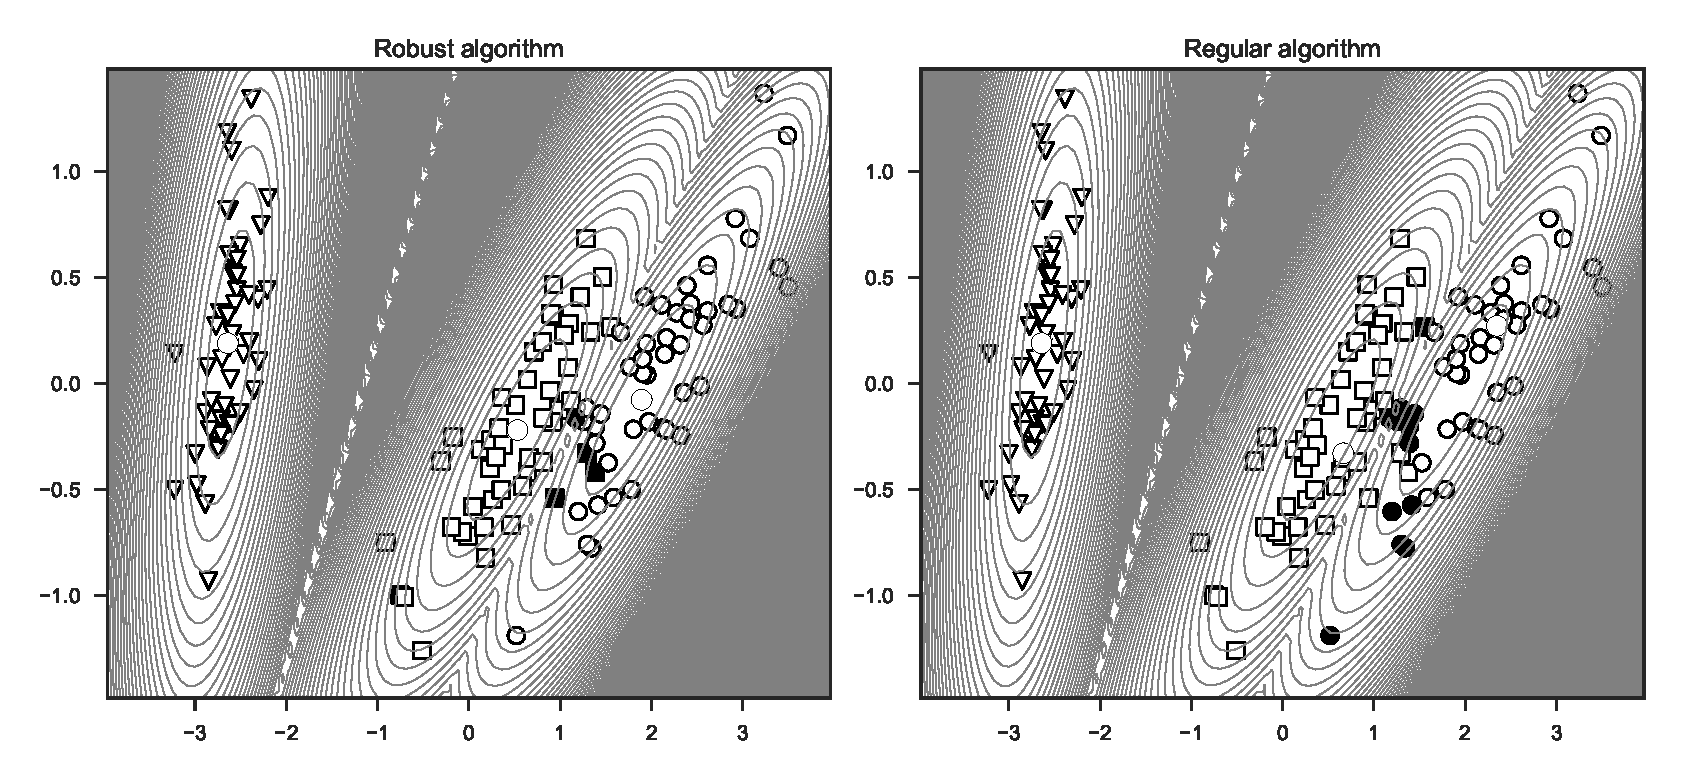
\includegraphics[width=1\columnwidth]{robust_kmeans_center_variance}\label{fig:iris}\caption{\textsf{IRIS}: Robust vs. regular algorithm. White markers correspond
to samples with the correct classes, black markers correspond to the
wrong classes.}
\end{figure}


\section{The algorithm}

To search $\mathbf{c}_{1}^{*},\dots,\mathbf{c}_{K}^{*}$ and $\mathbf{S}_{1}^{*},\dots,\mathbf{S}_{K}^{*}$
we apply an iterative scheme that corresponds to the analog of the
Jacobi method for solving the system of nonlinear equations \eqref{eq:eq_c_S}.

The initial positions of the centers are selected in some way, for
example: 
\[
\left\{ \begin{array}{l}
\mathbf{c}_{j,0}={\displaystyle \frac{1}{N}\sum\limits _{k=1}^{N}\mathbf{x}_{k}}\\
\mathbf{S}_{j,0}=\mathbf{E}^{n\times n},
\end{array}\right.
\]
where $\mathbf{E}^{n\times n}$ is identity matrix $n\times n$.
\begin{enumerate}
\item At the $t$-th step, two equations are successively solved:
\begin{enumerate}
\item For each $j=1,\dots,K$, the following vector equation is first solved
to find~$\mathbf{c}_{j,t+1}$: 
\begin{equation}
\mathbf{c}_{j}=\frac{1}{V_{j}}\sum\limits _{k\in\mathbf{I}_{j}}v_{k}\mathbf{x}_{k},\label{eq:eq_c}
\end{equation}
where $z_{k}=D_{k}(\mathbf{c}_{1},\dots,\mathbf{c}_{K};\mathbf{S}_{1,t},\dots,\mathbf{S}_{K,t})$.
\item Then, for each $j=1,\dots,K$, the following vector equation is solved
to find~$\mathbf{S}_{j,t+1}$:
\begin{equation}
\mathbf{S}_{j}=\frac{1}{V_{j}}\sum\limits _{k\in\mathbf{I}_{j}}v_{k}(\mathbf{x}_{k}-\mathbf{c}_{j,t+1})^{\prime}(\mathbf{x}_{k}-\mathbf{c}_{j,t+1}),\label{eq:eq_S}
\end{equation}
where $z_{k}=D_{k}(\mathbf{c}_{1,t+1},\dots,\mathbf{c}_{K,t+1};\mathbf{S}_{1},\dots,\mathbf{S}_{K})$.
\end{enumerate}
\item Step 1 is repeated until $t<T$ (maximum number of iterations) or
the sequence $\{\mathcal{Q}(\mathbf{c}_{t,1},\dots,\mathbf{c}_{t,K};\mathbf{S}_{t,1},\dots,\mathbf{S}_{t,K})\}$
will not concentrate around its condensation point.
\end{enumerate}
The sets of point indices $\mathbf{I}_{1},\dots,\mathbf{I}_{K}$ corresponding
to the partition into clusters are found before solving systems of
equations. An additional condition $|\mathbf{S}|=1$ is usually added
to prevent singularity of the covariance matrices. Scale factor $\sigma=|\mathbf{S}|$
can then be estimated using the $\mathsf{S}$-estimator~\cite{Dav1987}.

The first equation in the system has the form:
\[
\mathbf{c}=F(\mathbf{c}).
\]
To solve it, you can use the iterative procedure:
\[
\mathbf{c}_{t+1}=(1-h)\mathbf{c}_{t}+hF(\mathbf{c}_{t}),
\]
where $0\leqslant h\leqslant1.$ The second equation has a similar
form:
\[
\mathbf{S}=G(\mathbf{S}).
\]
To solve it, you can use a similar iterative procedure:
\[
\mathbf{S}_{t+1}=(1-h)\mathbf{S}_{t}+hG(\mathbf{S}_{t}).
\]


\section{Examples}

\begin{figure}
\noindent 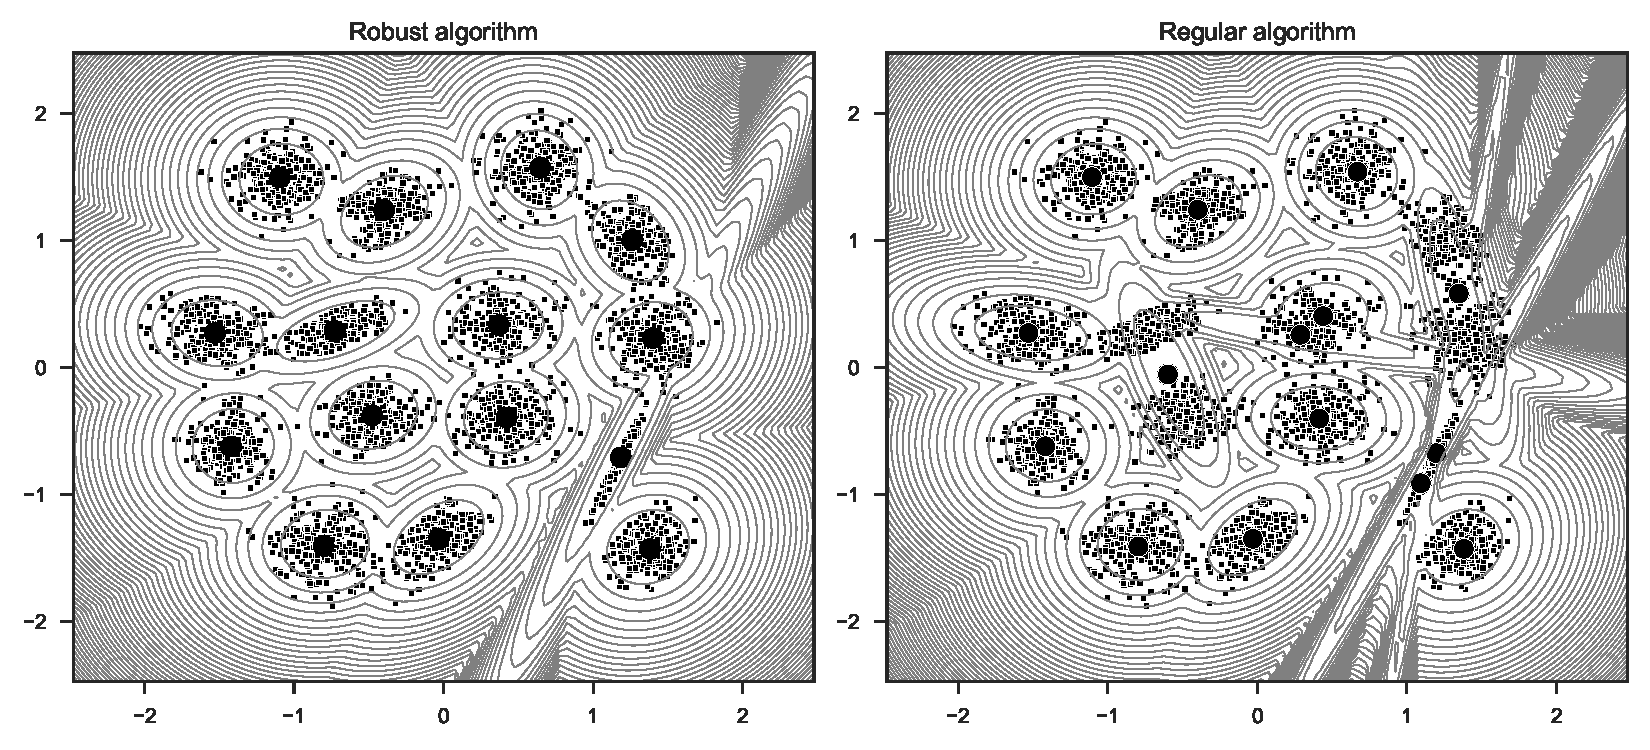
\includegraphics[width=1\columnwidth]{robust_kmeans_center_variance_s1}
\noindent \centering{}\caption{\textsf{S}1: The results of robust and classical algorithms.}
\label{fig:s1}
\end{figure}

\begin{figure}
\noindent 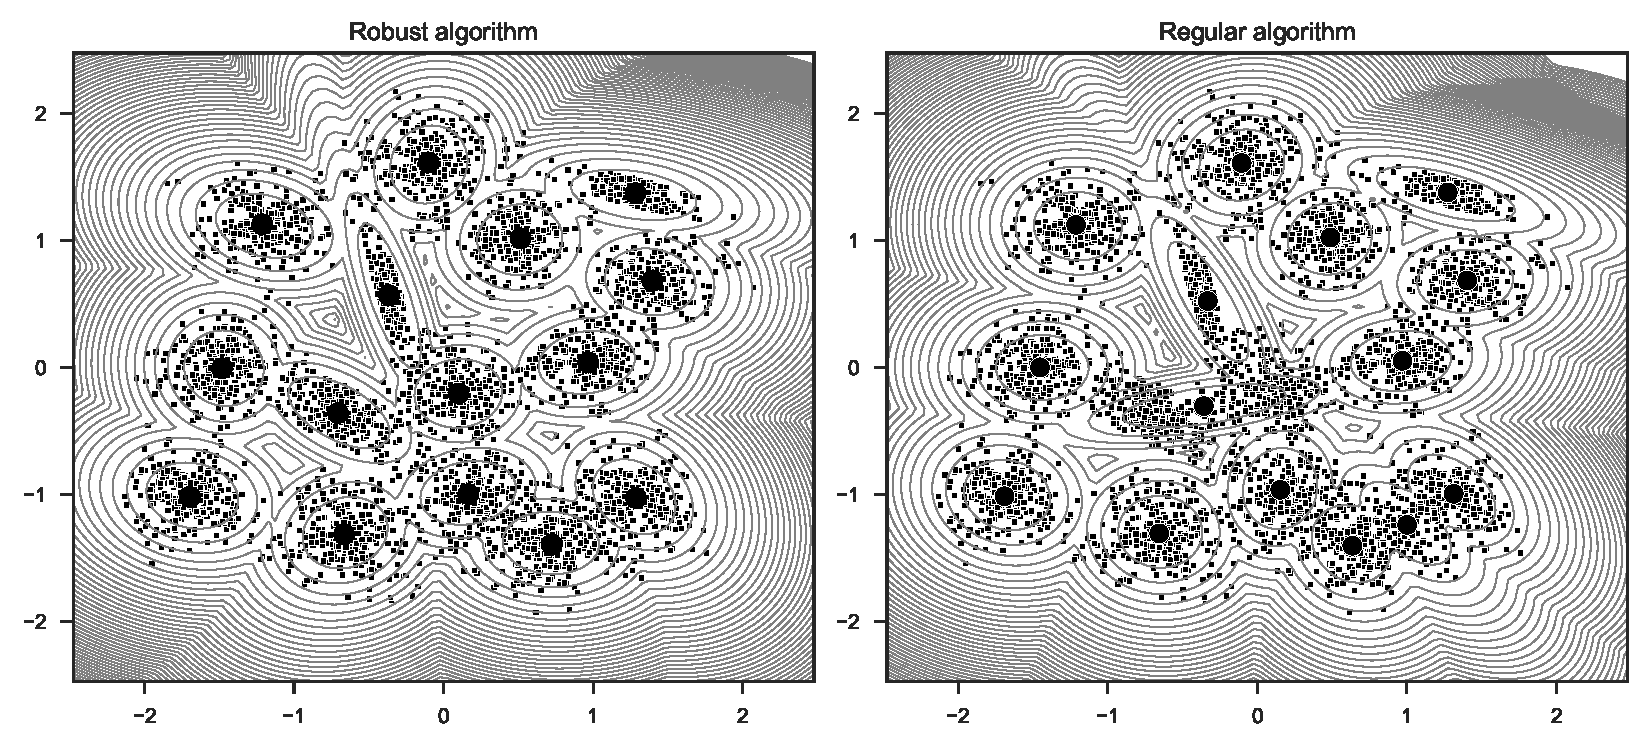
\includegraphics[width=1\columnwidth]{robust_kmeans_center_variance_s2}

\noindent \caption{\textsf{S}2: The results of robust and classical algorithms.}
\end{figure}

\begin{figure}
\noindent 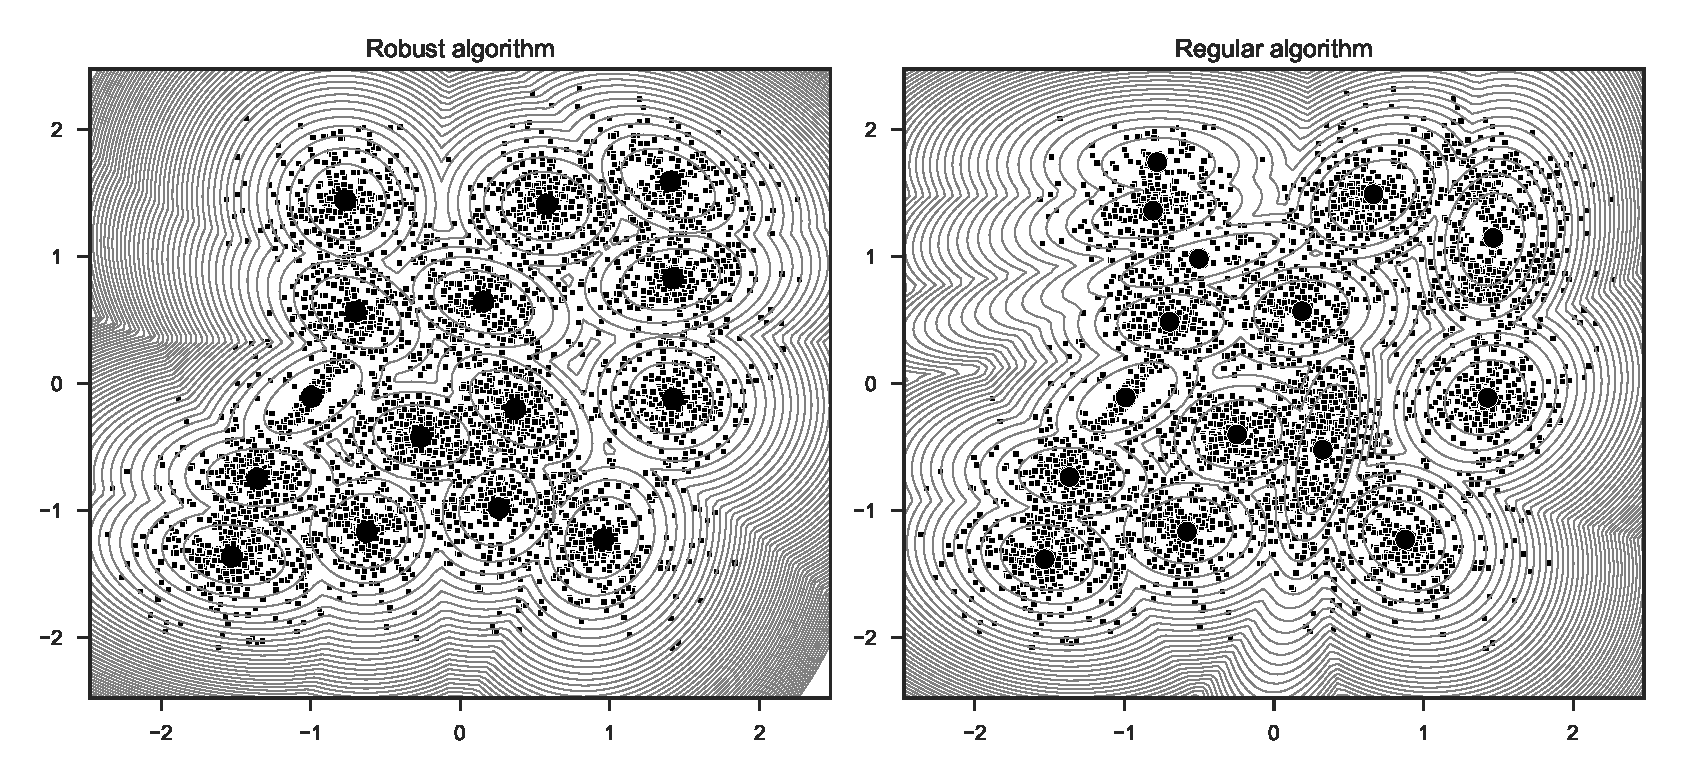
\includegraphics[width=1\columnwidth]{robust_kmeans_center_variance_s3}

\noindent \caption{\textsf{S}3: The results of robust and classical algorithms.}
\end{figure}

\begin{figure}
\noindent 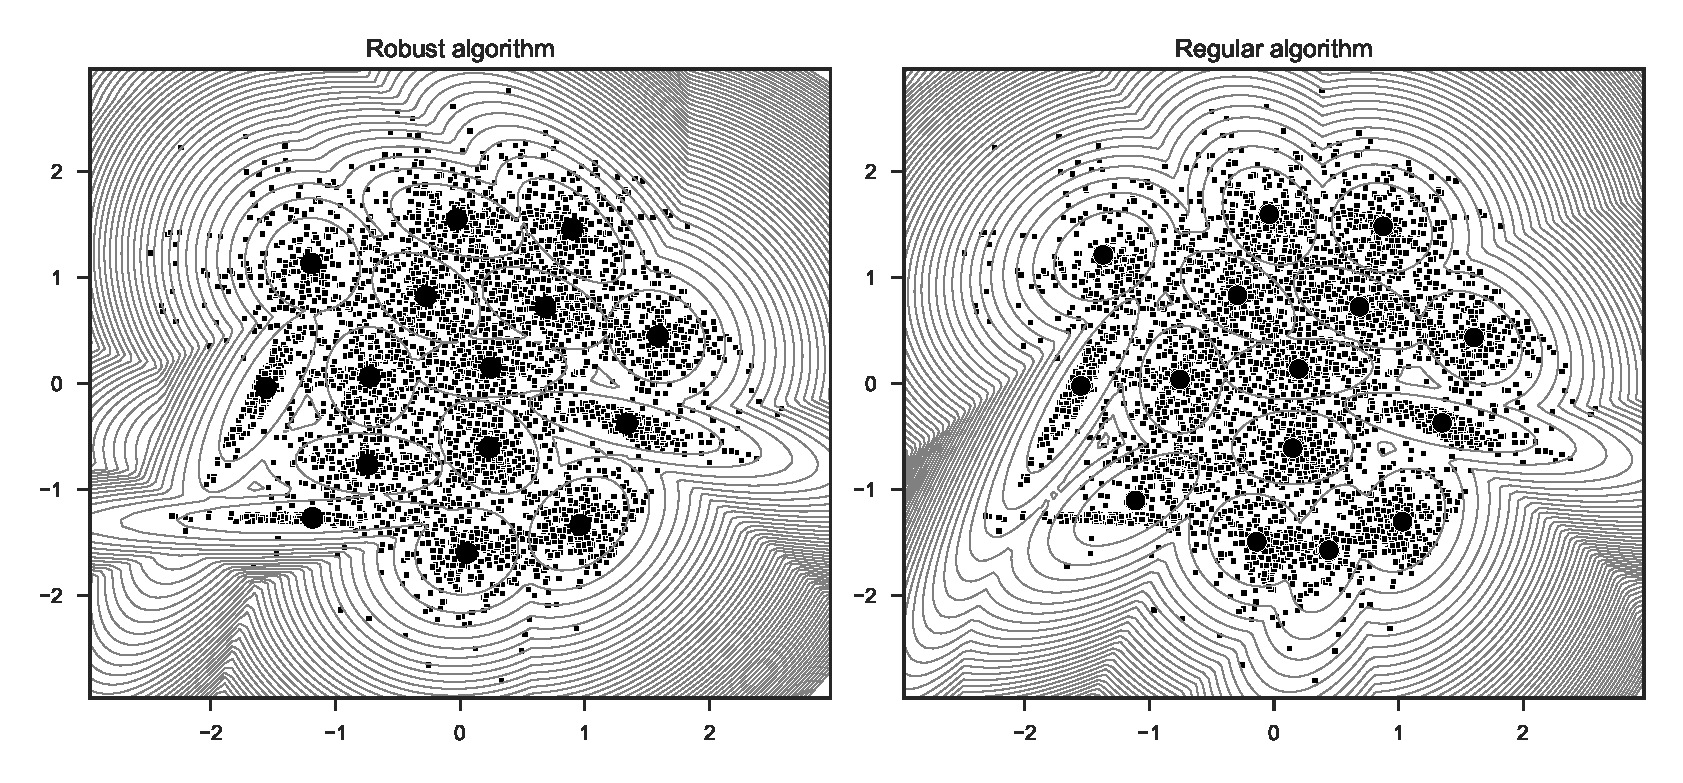
\includegraphics[width=1\columnwidth]{robust_kmeans_center_variance_s4}

\noindent \caption{\textsf{S}4: The results of robust and classical algorithms.}
\label{fig:s4}
\end{figure}


\subsection{IRIS dataset}

Consider the relatively simple and classic \textsf{IRIS} dataset (3
classes, 4 attributes, 150 items). Here we use data in projection
on 1st and 2nd principial components. As a rule, it is used for classification
tasks. Here we will try to identify classes using clustering, using
the Mahalanobis distance instead of Euclidean. Figure~\ref{fig:iris}
shows the results of clustering using the robust algorithm proposed
here and the classical algorithm. The result of clustering using the
robust algorithm (both using $\mathsf{WM}_{\rho_{\alpha}}$ and $\mathsf{TM}_{\rho_{\alpha}}$,
$\varepsilon=0.001$, $\alpha=0.96$) differs from the given classification
only at $3$ points out of $150$. The result of clustering using
the classical algorithm differs from the given classification in no
less than 6 points out of 150. For comparison, the classic \textsf{kmeans}
with Euclidean distance differs from the given classification at $17$
points out of $150$. This simple example shows that the application
of the proposed robust approach to clustering based on a realistic
set of features can allow us to construct a partition that differs
slightly from a given classification.

\subsection{Wine dataset}

Consider another classic \textsf{WINE} dataset (3 classes, 13 attributes,
178 items). As a rule, it is also used for classification tasks. Here
we will also try to identify classes using clustering, using the Mahalanobis
distance instead of Euclidean. The result of clustering using the
robust algorithm (both using $\mathsf{WM}_{\rho_{\alpha}}$ and $\mathsf{TM}_{\rho_{\alpha}}$,
$\varepsilon=0.001$, $\alpha=0.97$) differs from the given classification
only at 3--4 points out of 178. The result of clustering using the
classical algorithm differs from the given classification in no less
than 6--7 points out of 178. This simple example shows that the application
of the proposed robust approach to clustering based on a realistic
set of features can allow us to construct a partition that differs
slightly from a given classification.

\subsection{S1--S4 datasets}

Cosider datasets \textsf{S1--S4} for clustering from~\cite{SD2018,sdataset}.
They contain 5000 points, 15 clusters. In Fig.~\ref{fig:s1}--\ref{fig:s4}
presents the results of clustering for sets \textsf{S1--S4}, respectively.
On each figure, on the left side there is the result of the robust
algorithm, and on the right side there is the classical one. During
the training, a robust mean estimate was used with $\mathsf{TM}_{\rho_{\alpha}}$,
$\varepsilon=0.001$, $\alpha=0.96-0.97$, $h=0.95$. It is easy to
see that the robust algorithm allows one to find more adequate positions
of the centers of clusters and the shape of the variance matrices

\section{Conclusion}

In this paper, we considered a new variant of the \textsf{k-means}
algorithm, in which the Mahalanobis distance was used instead of the
Euclidean distance. The proposed new approach to constructing a robust
version of k-means algorithm with the Mahalanobis distance bases on
minimizing robust differentiable estimates of the mean. Its fundamental
resistance ability to strong distortions in data was shown compared
with the classical k-means algorithm. This is due to the fact that
the robust average estimates used in the work limit the influence
on the search for the position of the centers of clusters of points
that are located at relatively large distances from them. The differentiability
of the estimate of the average value, insensitive to outliers, allows
the use of gradient minimization algorithms to search for cluster
centers. Differentiability made it possible to construct an algorithm
based on the iterative reweighting method, so that at each step the
centers of the clusters are searched within the framework of the classical
k-means with sample weights. Taking into account the shape of the
covariance matrix significantly enhance the result. It should also
be noted that the result of the robust algorithm is not completely
stable. However, with a suitable choice of parameters $\alpha$ and
$h$, it can be achieved that in most starts of the training procedure,
an adequate result can be obtained.

\subsection*{Acknowledgments}

This work was supported by the RFBR grant No. 18--01--00050.
\begin{thebibliography}{10}
\bibitem{cp1}V.V.~Tatarnikov, I.A.~Pestunov and V.B.~Berikov,
``Centroid Averaging Algorithm for Building a Cluster Ensemble''.
Computer Optics. vol. 41 (5), pp. 712--718, 2017. DOI: 10.18287/2412-6179-2017-41-5-712-718.

\bibitem{cp2}A.K.~Jain, ``Data clustering: 50 years beyond K-means''.
Pattern Recognition Letters. vol. 31 (8), pp. 651-666, 2010. DOI:
10.1016/j.patrec.2009.09.011.

\bibitem{cp3}S.~Belim and P.~Kutlunin, ``Boundary extraction in
images using a clustering algorithm'' {[}In Russian{]}. Computer
Optics. vol. 39 (1), pp. 119--124, 2015. DOI: 10.18287/0134-2452-2015-39-1-119-124.

\bibitem{Mar1976}R.A.~Maronna, ``Robust M-Estimators of Multivariate
Location and Scatter'', Ann. Statist, vol. 4, pp.51--67, 1976. 

\bibitem{Rus2013}P.~Rousseeuw, M.~Hubert, ``High-breakdown estimators
of multivariate location and scatter'', In: Robustness and Complex
Data Structures. Ed.: C.~Becker, R.~Fried, S.~Kuhnt., Springer,
pp. 49--66, 2013.

\bibitem{Mar2015}R.A.~Maronna, V.J.~Yohai, ``Robust and efficient
estimation of multivariate scatter and location''. {[}Online{]}.
Available: arxiv:1504.03389, 2015.

\bibitem{sz2017}Z.M.~Shibzukhov, ``On the principle of empirical
risk minimization based on averaging aggregation functions''. Dokl.
Math., vol. 96 (3), pp. 494--497, 2017. \href{https://doi.org/10.1134/S106456241705026X}{https://doi.org/10.1134/S106456241705026X}

\bibitem{sz2019}Z.M.~Shibzukhov, M.A.~Kazakov, ``Clustering based
on the principle of finding centers and robust averaging functions
of aggregation'', Proceedings of V International Conference Information
Technology and Nanotechnology -- ITNT~2019. Journal of Physics:
Conference Series. {[}Online{]}. Avaliable: \href{https://iopscience.iop.org/article/10.1088/1742-6596/1368/5/052010/pdf}{https://iopscience.iop.org/article/10.1088/1742-6596/1368/5/052010/pdf}

\bibitem{Dav1987}P.L.~Davies, ``Asymptotic behavior of S-estimates
of multivariate location parameters and dispersion matrices'', Ann.
Statist, vol. 15, pp. 1269--1292, 1987.

\bibitem{SD2018}P.~Fr�nti, S.~Sieranoja, ``K-means properties
on six clustering benchmark datasets'', Applied Intelligence, vol.
48 (12), pp. 4743--4759, 2018.

\bibitem{sdataset}Clustering basic benchmark. {[}Online{]}. Available:
http://cs.joensuu.fi/sipu/datasets/
\end{thebibliography}

\end{document}
